% While writing, don't stop for errors
\nonstopmode

%%% This is based on the Frontiers template.
\documentclass{frontiersSCNS}

\usepackage{url,hyperref,lineno,microtype}
\usepackage[english]{babel}
\usepackage{amsmath}
\usepackage[onehalfspacing]{setspace}
\usepackage{gensymb} % For \degree

\linenumbers

% Trick to define a language alias and permit language = {en} in the .bib file.
% From: http://tex.stackexchange.com/questions/199254/babel-define-language-synonym
\usepackage{letltxmacro}
\LetLtxMacro{\ORIGselectlanguage}{\selectlanguage}
\makeatletter
\DeclareRobustCommand{\selectlanguage}[1]{%
  \@ifundefined{alias@\string#1}
    {\ORIGselectlanguage{#1}}
    {\begingroup\edef\x{\endgroup
       \noexpand\ORIGselectlanguage{\@nameuse{alias@#1}}}\x}%
}
\newcommand{\definelanguagealias}[2]{%
  \@namedef{alias@#1}{#2}%
}
\makeatother
\definelanguagealias{en}{english}
\definelanguagealias{eng}{english}
% End language alias trick


\def\keyFont{\fontsize{8}{11}\helveticabold }
\def\firstAuthorLast{James {et~al.}}
\def\Authors{Sebastian James\,$^{1,2,*}$, Chris Papapavlou\,$^5$, Alexander Blenkinsop\,$^{1,2}$, \\
  Alexander Cope\,$^3$,  \\
  Sean Anderson\,$^{2,4}$, Konstantinos Moustakas\,$^5$, Kevin Gurney\,$^{1,2}$}
% Affiliations should be keyed to the author's name with superscript
% numbers and be listed as follows: Laboratory, Institute, Department,
% Organization, City, State abbreviation (USA, Canada, Australia), and
% Country (without detailed address information such as city zip codes
% or street names).
%
% If one of the authors has a change of address, list the new address
% below the correspondence details using a superscript symbol and use
% the same symbol to indicate the author in the author list.
\def\Address{\\
$^{1}$Adaptive Behaviour Research Group, Department of Psychology,
  The University of Sheffield, Sheffield, UK \\
$^{2}$Insigneo Institute for in-silico Medicine,
  The University of Sheffield, Sheffield, UK \\
$^{3}$Department of Computer Science,
  The University of Sheffield, Sheffield, UK \\
$^{4}$Department of Automatic Control Systems Engineering,
  The University of Sheffield, Sheffield, UK \\
$^{5}$Department of Computer Science,
  The University of Patras, Patras, Greece \\
}
% The Corresponding Author should be marked with an asterisk. Provide
% the exact contact address (this time including street name and city
% zip code) and email of the corresponding author
\def\corrAuthor{Kevin Gurney}
\def\corrAddress{Department of Psychology, The University of Sheffield,
  Western Bank, Sheffield, S10 2TP, UK}
\def\corrEmail{k.gurney@sheffield.ac.uk}


\begin{document}

% A place for aliases:
% Aliases
\newcommand{\ccg}{Cope-Chambers-Prescott-Gurney}
\newcommand{\stob}{SpineML\_2\_BRAHMS}
% Emphasis and bold.
\newcommand{\e}{\emph}
\newcommand{\bol}{\textbf}

\newcommand{\blue}{\textcolor{blue}}

% I like my citations in blue
\newcommand{\mycite}[1]{\blue{\cite{#1}}}

% expon function is roman e
\newcommand{\expon}{\mathrm{e}}

% A font to indicate a branch of a github repository
\newcommand{\branch}[1]{\textbf{\texttt{#1}}}


\onecolumn
\firstpage{1}

\title[Integrated brain and biomechanics]{
Integrating brain and biomechanical models - a new paradigm
for understanding  neuro-muscular control
}

\author[\firstAuthorLast ]{\Authors}
\address{}
\correspondance{}
\extraAuth{} % If more than 1 corr. author refer to original template
             % and fill this in
%
%%%%%%%%%%%%%%%%%%%%%%%%%%%%%%%%%%%%%%%%%%%%%%%%%%%%%%%%%%%%%%%%%%%%%%%%%%%%%%%
%%% The sections below are for reference only.
%%%
%%% For Original Research Articles, Clinical Trial Articles, and
%%% Technology Reports the section headings should be those
%%% appropriate for your field and the research itself. It is
%%% recommended to organize your manuscript in the following sections
%%% or their equivalents for your field:
%%%
%%% Abstract, Introduction, Material and Methods, Results, and Discussion.
%%%
%%% Please note that the Material and Methods section can be placed in
%%% any of the following ways: before Results, before Discussion or
%%% after Discussion.
%%%
%%% For information about Clinical Trial Registration, please go to
%%% http://www.frontiersin.org/about/AuthorGuidelines#ClinicalTrialRegistration
%%%
%%% For Clinical Case Studies the following sections are mandatory:
%%% Abstract, Introduction, Background, Discussion, and Concluding
%%% Remarks.
%%%
%%% For all other article types there are no mandatory sections.
%%%%%%%%%%%%%%%%%%%%%%%%%%%%%%%%%%%%%%%%%%%%%%%%%%%%%%%%%%%%%%%%%%%%%%%%%%%%%%%
\maketitle
\begin{abstract}

\section{}
To date, realistic models of how the central nervous system governs
behaviour have been restricted in scope to the brain, brainstem or
spinal column, as if these existed as disembodied organs.
Further, the model is often exercised in relation to an in vivo
physiological experiment with input comprising an impulse, a periodic
signal or constant activation, and output as a pattern of neural
activity in one or more neural populations. Any link to behaviour is
inferred only indirectly via these activity patterns.
%
We argue that to discover the principles of operation of neural
systems, it is necessary to express their behaviour in terms of
physical movements of a realistic motor system, and to supply inputs
that mimic sensory experience. To do this with confidence, we must
connect our brain models to neuro-muscular models and provide relevant
visual and proprioceptive feedback signals, thereby closing the loop
of the simulation.
%
This paper describes an effort to develop just such an integrated
brain and biomechanical system using a number of pre-existing
models. It describes a model of the saccadic oculomotor system
incorporating a neuromuscular model of the eye and its six extraocular
muscles. The position of the eye determines how illumination of a
retinotopic input population projects information about the location
of a saccade target into the system.
%
A pre-existing saccadic burst generator model was incorporated into
the system, which generated motoneuron activity patterns suitable for
driving the biomechanical eye. The model was demonstrated to make
accurate saccades to a target luminance under a set of environmental
constraints.
%
Challenges encountered in the development of this model showed the
importance of this integrated modelling approach. Thus, we exposed
shortcomings in individual model components which were only apparent
when these were supplied with the more plausible inputs available in a
closed loop design. Consequently we were able to suggest missing
functionality which the system would require to reproduce more
realistic behaviour.
%
The construction of such closed-loop animal models constitutes a new
paradigm of {\em computational neurobehaviour} and promises a more
thoroughgoing approach to our understanding of the brain's function as
a controller for movement and behaviour.

\tiny
 \keyFont{
   \section{Keywords:}
   integrated brain biomechanics neuromuscular oculomotor saccade basal ganglia
 } % 5 to 8 keywords
\end{abstract}

\section{Introduction}

% New introduction, tailored to the paradigm shift title.
(New Introduction:)

The field of computational neuroscience has provided
many \e{systems models} of the brain~\cite{arai_two-dimensional_1994,gancarz_neural_1998,hazy_towards_2007,blenkinsop_frequency_2017}. We
refer to these as \e{mechanistic computational models}, meaning
models which consist of populations of neural elements, interconnected
in a biologically plausible manner, which simulate the operation of
the brain.

Whilst they differ in scale and complexity, these models all seek to
describe the fundamental mechanisms behind common animal behaviours
such as locomotion, threat evasion, reaching or feeding. However,
almost none of the models cited here actually reproduce these
behaviours. In each case, the activity in a certain population of
neurons is taken to be representative of a behavioural outcome.


%%%%%%%%%%%%%%%%%%%%%%%%%%%%%%%%%%%%%%%%%%%%%%%%%%%%%%%%%%%
(Old introduction, which became the VPH mini-paper intro:)
%%%%%%%%%%%%%%%%%%%%%%%%%%%%%%%%%%%%%%%%%%%%%%%%%%%%%%%%%%%

% Can make comparisons
As mechanistic computational models of brain systems become more
sophisticated we can aspire to make realistic comparisons between the
behaviour of the model and that of the animal or human.

% Short desc of mechanistic computational model
By \e{mechanistic computational model}, we mean a model which
consists of populations of neural elements, interconnected in a
biologically plausible manner. Such a model may consist of neural
elements that produce a time-dependent membrane voltage and realistic
spiking behaviour (Hodgkin-Huxley, Fizhugh-Nagumo, Izhikevich, Leaky
integrate and fire) in which case the neural element's activity can be
obtained by counting action potentials (or considering their
timing). Alternatively it may (as it does in this work) consist of
rate-coded neural elements, whose activation variable is related to
the spiking rate of a number of neurons (refs).

% Sometimes, ok to just have a brain model
In some cases, it is sufficient to take the activity of an internal
population within the brain model as being representative of the
induced behaviour. For example, a choice made in a \e{go/no-go} task
could be determined from activity in a population within a Basal
Ganglia model
(\cite{nambu_discharge_1990,kuhn_event-related_2004}). The decision
to \e{go} is selected by a reduction of activity in this population;
maintenance of activity implies \e{no-go}. Error rates in this task
could be compared with experimentally determined error rates in
primate subjects.
% Brain model comparison validates model
If the expression of behaviour by the model is similar when compared
with the experimental data, this serves to validate the model for the
healthy, neuro-typical subject.
% Now describe comparison between model and expt. for diseased
% subject.
If we have confidence in the model's description of the behaviour for
the healthy subject, we can now progress to a comparison between the
model and an unhealthy subject. If we can identify a characteristic
degradation in an aspect of the brain for an unhealthy subject, then
we can seek to modify the model to mirror this degradation. By
comparing the relationship between the model's behaviour as a function
of the degradation parameter with the unhealthy individual's behaviour
as a function of disease progression, we may be able to relate the
disease progression state to the brain parameter and predict the
time-course of the internal degradation of the brain.
% Leave further discussion along these lines to the discussion
% section.

% But sometimes you might need brain and neuromuscular model
Many behaviours are more complex and subtle than a decision. In the
disease state, it may be the dynamics of the movement which is
symptomatic rather than its outcome. A diagnostic task may produce an
outcome whose error rate varies with disease state, but it may also
produce movement characteristics which correlate with the disease
progression such as the slow, jerky or inaccurate movements seen in
Parkinson's Disease. In order to determine the validity of a model
which seeks to describe more complex movements, it is necessary to
express the movement commanded by the brain network as a realistic,
simulated motion by means of a biomechanical model, driven by the
brain model.

% Motivation here is to study movement disorders by means of a
% comparison between healthy subjects, the healthy model and diseased
% subjects and the diseased model.
Our motivation is to study movement disorders using our brain
models. Because the challenge of integrating brain and biomechanical
models has not, to our knowledge, previously been addressed, we chose
to express some of the simplest, and most studied movements made by
vertebrates: the rapid eye movements known as saccades. Saccades
direct the fovea, the region of the eye with the highest spatial
imaging resolution, towards putative targets of interest. Mammals make
frequent saccades; many thousands every day. These movements are often
described as ballistic: They are commanded by activity in the superior
colliculus which encodes an endpoint for the saccade trajectory
(\cite{wurtz_superior_1971,hepp_monkey_1993}); once initiated, the
saccade proceeds in a relatively direct and stereotyped (though not
always straight) trajectory (\cite{van_der_stigchel_eye_2006}) to
the endpoint.
% Why am I mentioning curved saccades? Because it shows that saccades
% can exhibit rich behaviour and that modelling them is worthwhile.
However, numerous studies have shown that saccade trajectories are
affected by distractors (\cite{mcpeek_competition_2003,
port_sequential_2003, van_der_stigchel_recent_2010}) and may be
modified in-flight to the extent that saccades may be seen to perform
significant, sometimes even U-shaped, curves towards or away from
distractors. This shows that whilst saccades are simple compared to
the movements of limbs, they still provide information about a number
of mechanisms within the brain and an effort to model them accurately
is worthwhile.

% Say what we've done here, in short form.
Parkinson's Disease is a progressive neurological disorder whose main
symptoms relate to motor control. These include resting tremor,
slowness of movements (bradykinesia), difficulty in initiating
movement (akinesia) and rigidity (refs). It is considered to be a
disease of the basal ganglia because during its progression, dopamine
producing neurons in the substantia nigra pars compacta die away
(ref), affecting the the striatum which depends on endogenous dopamine
for correct operation (ref). The basal ganglia plays an important role
in decision making and action selection (ref), including the selection
of saccadic eye movements (\cite{hikosaka_role_2000}). In the later
stages of Parkinson's Disease, patients show more latent saccades to
targets of interest (ref). They have also been documented as showing
poorer performance in the so-called anti-saccade protocol, in which
the subject is instructed to make a saccade \e{away} from a visual
target. Parkinson's Disease patients make significantly more errors;
they will saccade \e{to} the visual target rather than \e{away} from
it more often than healthy control subjects. To investigate the way in
which degradation in the basal ganglia may be causing these defects we
have developed an integrated brain and biomechanical eye model which
we describe here. The model will initially be used to investigate the
deterioration in anti-saccadic movements which is detectable even in
relatively early-stage Parkinson's Disease.

%See \cite{Rottach_dynamic_1996} for trajectory information in saccades.

%% End of intro here? Or carry on with a description of the physiology
%% of saccadic eye movements?

Many neural populations are involved in the coding of saccadic eye
movements, only a very brief overview is given here; for a recent
review, see \cite{munoz_commentary:_2002}. One pathway takes
information from the retina directly into the superficial layers of
the superior colliculus in the brainstem (\cite{sterling_receptive_1971,linden_massive_1983,wu_involvement_1994}).
Activity within
the superior colliculus then excites neurons in the pons, medulla and
rostral mid-brain (\cite{sparks_brainstem_2002}) and then through
channels to the motor neurons which innervate the extraocular muscles
(\cite{fuchs_firing_1970,sparks_brainstem_2002}). This direct pathway
is responsible for the low latency saccades called express saccades
(\cite{schiller_effect_1987,edelman_activity_1996}).

% FEF: \cite{schall_neural_1999}
Information from the retina is also processed by visual cortex which
feeds through to the frontal eye fields in which activity is related
to reflexive and voluntary
saccades \cite{schall_neural_1999}. Activity build up in the frontal
eye fields is transferred to the intermediate layers of the superior
colliculus
\cite{stanton_frontal_1988-1} and is also processed by the basal ganglia, which
participates in the selection of the winning saccade end point
\cite{stanton_frontal_1988}.

% On fact that SC doesn't encode oblique/torsional movements:
% \cite{hepp_monkey_1993}

% That means that you need both the expression of movement, and also a
% means by which you can progress the disease in the model.

%If such comparisons are to be made, then the behavioural output of the
%model should be in the form of movements which can be directly
%compared with the biological system. In order to express movements,
%the brain model needs to drive biomechanical neuromuscular models.


%\begin{methods}
\section{Material \& Methods}

% A very short introduction to the section.
The integrated brain and biomechanical model described here is a
development of the model in \cite{cope_basal_2017},
referred to here as the \ccg~model. This was a rate-coded neural
network model incorporating retinal populations, frontal eye fields
(FEF), the basal ganglia (BG), and the superior colliculus (SC). In
the \ccg~model, the centroid of the activity in the deep
layers of superior colliculus was assumed to accurately encode the
location of the eye at the end of the
saccade~(\cite{wurtz_activity_1972,robinson_eye_1972,van_gisbergen_collicular_1987,mcilwain_lateral_1982}).
This location was used to recalculate the positions of the luminances in
the eye's frame of reference at each time step. The model included no
brainstem populations other than superior colliculus, nor a
neuromuscular model.

To summarize, the \ccg~model takes as \e{input} the positions
of luminances on a topographic map and produces as output a saccade 
target.

To the \ccg~model, we have added a rate-coded brainstem model (a ``saccadic
burst generator''), and a biomechanical eye, implemented using the
biomechanical modelling framework OpenSim. These will be described below,
but first we will give a description of the co-ordinate systems and the
modelling framework used.

\subsubsection{Coordinates in the world}

Before describing the biomechanical eye and the brain model, which consisted
of retinotopically mapped neural sheets, we describe the coordinate system
used in the world. The eye was located at the origin of a 3 dimensional, right-handed 
Cartesian co-ordinate system, with its fovea directed in the $-z$ direction. 
There was a notional spherical screen which was also centered at the origin of the
co-ordinate system and had a radius of 50 (in arbitrary units). The \e{fixation 
point} was the point on the
screen at which the eye was initially directed.
Onto the screen were projected luminances, each of which having a position 
described by two co-ordinates; $\theta_x$, a 
rotation of the horizon plane about the $x$ axis, and $\theta_y$, a rotation 
of the meridian plane about the $y$ axis. The position is the intersection
of these rotated planes with the spherical screen (disregarding
the intersection point of these three surfaces behind the eye).
%
Note that a luminance with positive $\theta_x$ was above the horizon of this world; 
one whose $\theta_y$ was positive lay to the left of the world's meridian.

Luminances were crosses of height and width subtending 6$\degree$ and whose
`bars' were 2$\degree$ thick. Luminances were oriented like $+$ symbols with
their vertical bar aligned with the meridian plane and their horizontal bar 
aligned with the horizon plane described above.

The eye's frame of reference was initially aligned with the world's frame
of reference. 
At each timestep, the eye's rotational state ($R_x$, $R_y$, $R_z$) was 
used to translate the three dimensional
Cartesian co-ordinates of the luminances in the world frame into co-ordinates
in the eye frame. The luminance coordinates in the eye's frame of reference
were used to determine the input to the brain model.

% Section - description of how the model fits together - which
% components it's made from.
\subsection{Model development framework}

% Say the \ccg~model was implemented in matlab-brahms & this one is SpineML.
The \ccg~model was originally developed to run on the BRAHMS model
execution framework
(\cite{mitchinson_brahms:_2010,mitchinson_brahms_2015}). To run a
BRAHMS model, the researcher must develop \e{BRAHMS components} for
the various neural elements. A BRAHMS component is a programmatically
coded implementation of the behaviour of the component. It may have an
arbitrary number of inputs and outputs and may be written in C, C++,
Python or MATLAB. The \ccg~model's components were hand written in C++
and MATLAB. A BRAHMS \e{SystemML} file describes how the different
components connect together and how data is passed between them
(\cite{mitchinson_brahms:_2010}). The main BRAHMS program first
reads the SystemML file, then dynamically loads all the required
components before executing the system.

In the current work, the \ccg~model was reproduced using the
declarative SpineML markup language (\cite{richmond_model_2014}),
with the help of the graphical SpineML model editing software
called SpineCreator
(\cite{cope_spinecreator:_2016}). SpineML,
which is a development of the NineML specification
(\cite{incf_task_force_on_multi-scale_modeling_network_2011}),
describes neural populations and their projections in a highly
structured format in which neuron bodies, pre- and post-synapses are
described in terms of \e{SpineML components}. These are similar to the
components provided by BRAHMS, but in this case, the components are an
XML description of the functionality of the component, rather than a
programmatic implementation, with one XML file per component. A
SpineML \e{network layer} file then describes which components are
used in the model, and how they are connected together. Finally, a
number of SpineML \e{experiment layer} files specify how the model
described in the network layer can be executed. In the experiment
layer, the execution duration and timestep can be specified, along
with input conditions, connection lesions and component parameter
updates. A complete description of SpineML is given
in \cite{richmond_model_2014}.

SpineCreator, in its r\^ole as a graphical editor for the SpineML
format, was used to generate the SpineML files describing the
model. It was also used to generate the diagrams of the model
(e.g. Fig.~\ref{fig:brain_model}).

As a declarative format for model specification, SpineML is agnostic
about how the model is executed. A number of simulation
engines can be utilised, including DAMSON (\cite{richmond_damson_2015}), GeNN
(\cite{nowotny_flexible_2011,nowotny_spineml_2014}) and BRAHMS (used
here). The simulation engine incorporating BRAHMS is called \stob~
(\cite{cope_spineml_2_brahms_2015-1}). \stob~is a collection of XSLT
stylesheets which first generate and compile C++ BRAHMS components
from the SpineML component layer description files. \stob~then uses
the SpineML network and experiment layer files to generate a BRAHMS
SystemML description of the model. Finally, \stob~executes the model,
now described entirely as a BRAHMS system, via a call to the BRAHMS
binary. A number of additional hand-written components are present
in \stob~providing the inputs (constant inputs, time-varying inputs,
etc) which the modeller specifies in the experiment layer.

In addition to the brain model components, all of which are
code-generated using \stob~as described above, two hand-written
components are integrated into the model: The biomechanical eye model
and a sensory input component. The sensory input component takes the
eye's rotational state and the state of the experimental luminances
and projects a retinotopic activity map into the brain model. Both of
these BRAHMS components were hand-written in C++. To incorporate these
components into the SpineML model, a model-specific modification was
applied in \stob~(\cite{cope_spineml_2_brahms_2015}) making use of
a \stob~feature designed for this purpose (The external.xsl file).

Figure \ref{fig:model_framework} shows the workflow, in which the
model specification files (blue box - a combination of SpineML files
and C++ code), are processed (green box) into a BRAHMS system (red
box).

\subsection{Existing brain model}

The brain model, excluding the brainstem, is a re-implementation of
the \ccg~model. Figure \ref{fig:brain_model} shows the layout of the
populations and the interconnections between them. Each population of
2500 elements is arranged as a 50 by 50 grid which forms a map in a
retinotopic co-ordinate system, roughly matching the known layout of
the superior colliculus~(\cite{robinson_eye_1972}). % FIXME: and frontal eye field?

\subsubsection{Components}

With the exceptions of the World and FEF\_add\_noise populations, each
neural element represents an activation; the activation is governed by
a first order differential equation specified in the SpineML
component. In the brain model, there are six different components in
use: LINlinear; LINret; LINexp; D1MSN and D2MSN.

The LINlinear component governs the activation $a$ with a first order
leaky integrator differential equation:
\begin{equation}
   \dot{a} = \frac{1}{\tau}(a_{in}-a)
\end{equation}
where $\tau$ is the time constant for the neural activation and
$a_{in}$ is the input to the neural element. $a_{in}$ is defined by an
activation input and a shunting inhibition input according to:
\begin{equation}
   a_{in} = A(1-s_a)+\alpha R_N
\end{equation}
Here, $A$ is the activation input and $s_a$ is the shunting inhibition
state variable whose value is related to the shunting input, $S$ by
\begin{equation}
   s_a = \begin{cases}
      S & S\leq 1 \\
      1 & S > 1
   \end{cases}
\end{equation}
$R_N$ is a random number drawn from a standard normal distribution
($\sigma$=1, $\mu$=0) and introduces noise to the activation of the
neural element, with the parameter $\alpha$ controlling the noise
amplitude.

The output, $y$, of LINlinear is related to the activation $a$ by the
piecewise linear transfer function
\begin{equation}
   y(a) = \begin{cases}
      0   & a < c \\
      a-c & c \leq a \leq 1+c \\
      1   & a > 1+c
   \end{cases}
\end{equation}
where $c$ is a parameter defining the slope of the transfer
function. At this point, the naming scheme for the component becomes
apparent; this is a Leaky Integrator with a linear transfer function.

The LINret component used for the retinal populations is again similar
to the LINlinear component, but with no intrinsic noise and no
shunting inhibitory input. It has a neural input which is identical to
the activation input $A$:
\begin{equation}
   a_{in} = A
\end{equation}
The LINexp component is a leaky integrator with an exponential
transfer function. It shares the same differential equation with
LINlinear, but has a different input equation and a different output
transfer function. It has the following equation for the neural
element input $a_{in}$:
\begin{equation}
   a_{in} = [A+N(a-V_{r}^{-})] (1-S) + 0.01 R_N
\end{equation}
where $A$ is the activation input and $N$ is an input which is
modulated by $V_{r}^{-}$, a reversal potential, and $a$, the current
activation of the element. These inputs are summed and then reduced by
a factor which is dependent on $S$, the shunting input. As in
LINlinear, $R_N$ introduces normally distributed noise to the element.

The output, $y$, of the LINexp component is given by
\begin{equation}
   y(a) = \begin{cases}
      \mathrm{e}^{a}-0.9   & \mathrm{e}^a \leq 1+0.9 \\
      1   & \mathrm{e}^a > 1+0.9
   \end{cases}
\end{equation}
This component is used in the STN population, as it gives a more
physiologically accurate f-I
behaviour \cite{wilson_model_2004,bevan_mechanisms_1999,hallworth_apamin-sensitive_2003}
which has been shown to allow the mapping of the basal ganglia network
architecture onto an optimal decision making
model \cite{bogacz_basal_2007}.

The D1MSN and D2MSN components are both leaky integrators, similar to
LINlinear. They differ in that they have no shunting inhibition and a
dopamine parameter that modulates the input activation, so
that their equations for $a_{in}$ are thus:
\begin{equation}
   a_{in}^{D1} = (0.2 + d)A + 0.01 R_N
\end{equation}
\begin{equation}
   a_{in}^{D2} = (1 - d)A + 0.01 R_N
\end{equation}
where $d$ is a dopamine parameter. Varying dopamine from 0 to 1
enhances the activation in the D1 model, whereas it decreases
the activation of the D2 model elements, in line with experimental
observations~\cite{refs}. Note that the equation for $a_{in}^{D1}$
differs from that used in the \ccg~model, for which the
cortico-striatal weights are multiplied by $(1+d)$ rather than
$(0.2+d)$.

The equations given above are applied to each element in a
population. The value of the activation $A$ (and where relevant, the
shunting input, $S$) is determined by summing the weighted
inputs to the population:
\begin{equation}
A = \sum_{i}w_i^{act} x_i^{act}
\end{equation}
\begin{equation}
S = \sum_{i}w_i^{sh} x_i^{sh}
\end{equation}

%
% That's the components described. Next up is to have a figure of the
% activity for representative input to the model.
%

\subsubsection{Population activity and retinotopic mapping}

Each population of 2500 neural elements was arranged in a 50 by 50
grid, with positions on the grid representing a retinotopic
mapping similar to that found empirically both in the superior 
colliculus (\cite{ottes_visuomotor_1986}) and in visual cortex (\cite{eric_l._schwartz_computational_1980}) and assumed in
this work to persist throughout the oculomotor system.

In a retinotopic mapping, the Cartesian coordinates of the light-sensitive
cells in the retina, whose density varies with distance from the fovea,
are transformed into the Cartesian co-ordinates of 
the correspondingly active cells on the colliculus. The mapping ensures 
that an even density of cells can be maintained in the colliculus, but 
ensures that a single group of proximal, active, retinal neurons will 
always activate a single, proximal group of neurons on the collicular 
surface.

The mapping turns out to resemble polar coordinates. That is, one 
axis of the collicular surface specifies the eccentricity of
a retinal location (how far it is from the fovea) and the second axis
specifies the rotational angle of the retinal location; we therefore
use the convention 
of referring to the eccentricity axis on the colliculus as $r$ and the 
rotation axis as $\phi$.

The \e{cortical magnification factor}, $M(r)$, gives the relationship
between the
radial eccentricity $r$ and the retinal neural density. As in 
\cite{cope_basal_2017}, we use a first-order approximation of the form
for $M(r)$ given in  \cite{rovamo_estimation_1979}:
\begin{equation} \label{eq:cmf}
M(r) = \frac{M_f}{1+\frac{r}{E_2}}
\end{equation}
The foveal magnification, $M_f$, is the magnification of the most central
region of the retina and has a value in the human of about
7.8 mm/$\degree$~\cite{rovamo_estimation_1979}.

In our model, $M_f$ is related to $W_{nfs}$, the width of the retinotopic neural 
field, $W_{fov}$, the width of the eye's field of view and $E_2$, the 
eccentricity at which the retinal density has halved by:
\begin{equation} \label{eq:fm}
   M_f = \frac {W_{nfs}} {E_2\;\ln\left(\frac{W_{fov}}{2 E_2} + 1\right)}
\end{equation}
Here, $W_{nfs}$ is 50, $W_{fov}$ is set to 61$\degree$, a
reduction from the biophysically accurate 150$\degree$ due to the small
number of neurons in the retinotopic neural field. $E_2$ is
2.5~\cite{cope_basal_2017,slotnick_electrophysiological_2001}.

The mapping from the retinotopic co-ordinates $r$ and
$\phi$ to rotational co-ordinates $\theta_x$  and $\theta_y$ on
the retina was written
down by \cite{eric_l._schwartz_computational_1980} for striate cortex and 
\cite{ottes_visuomotor_1986} for superior colliculus. We used the following
statement of this mapping for all of the populations in
the brain model:
\begin{equation}
   \theta_x = E_2 \left(e^{\frac{r}{M_f E_2}} - 1\right).\cos\left(\frac{2 \pi \phi}{W_{nfs}}\right)
\end{equation}
\begin{equation}
   \theta_y = E_2 \left(e^{\frac{r}{M_f E_2}} - 1\right).\sin\left(\frac{2 \pi \phi}{W_{nfs}}\right)
\end{equation}

Note that the mapping encompases the entire visual field. The value of
$\phi$ is allowed to vary from 0$\degree$ to 360$\degree$ along its axis.
Effectively, the two contralateral colliculi found in the biology are 
incorporated into a
single, square map, avoiding the need to carry out the kind of `colliculus
gluing' described in \cite{tabareau_geometry_2007}.

It is straightforward to show that the reverse mapping is given by:
\begin{equation}
   \phi = \frac{W_{nfs}} {2 \pi}\arctan\left(\frac{\theta_y}{\theta_x}\right)
\end{equation}
\begin{equation}
   r = M_fE_2\,\ln\left(\frac{1}{E_2}\sqrt{{\theta_x}^2 + {\theta_y}^2}+1\right)
\end{equation}

Figure \ref{fig:mapping} shows the result of the mapping for a view of
two cross-shaped luminances. One cross illuminates the fovea, which
results in a large comb-shape of activity. The more peripheral cross
produces (in FEF) an indistinct object centered at a larger value of
$r$.

\subsubsection{Network}

Briefly, the model consists of input from the World population (see
Fig.~\ref{fig:brain_model}, green population box) producing activity
in an `express' pathway to superior colliculus (purple) and
simultaneously in cortex, represented here by the FEF population (grey
boxes in Fig.~\ref{fig:brain_model}). The express pathway causes short
latency activity in the superficial superior colliculus, which
directly innervates the deeper layers of the superior colliculus
(SC\_deep). Activity in FEF generates firing in a
thalamo-cortico-basal ganglia loop. The output of the basal ganglia is
the substantia nigra pars reticulata (SNr) which tonically inhibits
SC\_deep. If a location of activity in FEF is able to dominate
selection in the basal ganglia circuit, the corresponding location in
SNr will dis-inhibit and activity will build up in SC\_deep encoding
the saccade end point.

Connections shown in red are one to one connections; dark blue
projections indicate a connectivity pattern which `fans out' with a
2-D Gaussian kernel; lighter blue connections from STN to SNr and GPe
are diffuse, all-to-all connections and projections coloured green are
one-to-one connections that decay towards the fovea so that foveal
activity in FEF does not swamp the basal ganglia which would prevent
peripheral luminances from ever being selected.

Note that SC\_deep contains two recurrent connections; one is
excitatory, with a Gaussian kernel mapping and the other implements
tecto-tectal inhibition, which increases the inhibition between
activity in opposite hemispheres of the field of view (refs) helping
to resolve competition between saccades to the left and right. The
tecto-tectal inhibitory connection is \e{not} present in
the \ccg~model. In all other respects the model is as described in 
\cite{cope_basal_2017}.

%However, it does not describe deeper, motor regions of the
%brainstem, instead regarding the centroid of the activity in SC as
%being representative of the end point of the saccade
%trajectory \cite{mays_dissociation_1980,lee_population_1988,van_Opstal_role_1990}.

% Section - description of new brainstem model
\subsection{brainstem model}

In this model, we implement a saccadic burst generator (SBG) based
on \cite{gancarz_neural_1998}. The SBG network for two of the model's
six channels is shown in Fig.~\ref{fig:sbg}. Activity from the output
layer of superior colliculus (SC\_avg) is fed into each channel, which
sums the activity it receives and processes it in populations each of
a single neural element representing all the neurons in that
population.

Neurons in the deep
layers of the superior colliculus called long lead burst neurons
innervate excitatory burst neurons in the reticular formation (REF,
and check if LLBNs are really in SC).

Alex B to write this section?

Note that inhibition from IBN populations is fed back - or is this
detail for the `integration' subsection?

% Section - description of biomechanical model
\subsection{biomechanical eye}

% Possibly introductory paragraph here.

% Patras - what about a figure here?

% EYE MODEL DESCRIPTION HERE
The biomechanical eye model, implemented using the OpenSim framework
\cite{seth_opensim:_2011}, is anatomically represented by a sphere of
uniform mass distribution. The diameter of the eye is 24 mm for adults,
with small variations between individuals; the mass of the eye is 7.5 grams.
The eyeball is actuated by six extraocular muscles
(EOMs). The EOMs are arranged in three pairs forming a cone inside the
orbit with the apex being located inside the cranium in a tendonous
ring called the annulus of Zinn. An important feature of the
oculomotor system which greatly affects its overall behavior is the
existence of dynamic EOM pulleys. Their role is to guide the pivot
point of the EOMs. In our model, a pulley for each EOM has been
modeled by a point on the orbit whose location depends on the current
eye orientation.

%EOM dynamics
The force applied by EOMs is controlled by an excitatory signal
supplied by motoneurons in the brainstem. The dynamics of muscular
forces can be split into: 1) The elasticity of the muscles. 2) A delay
between the onset of the afferent excitatory signal and the actual
muscle contraction, caused by the transmission time of the action
potentials and by the necessary calcium release at the muscle
fibres. We developed a custom extraocular muscle model which captures
these features.

%Orbital fat force
Passive forces due to the fatty tissues inside the eye orbit also
affect eye dynamics. Their role is critical in eliminating the
influence of head and body movements. We incorporated a custom torque, $\mathbf{t}$,
which acts like a rotational spring-damper apparatus, resisting
eyeball movements. It has elastic and viscous properties governed by
$\mathbf{t} = -K\mathbf{R}-C\mathbf{U}$ where $\mathbf{R}$ is the
eye's orientation and $\mathbf{U}$ is its angular velocity. $K$ and
$C$ are constants. A fuller description of the biomechanical model 
can be found in \cite{papapavlou_physics-based_2014}.

% Section - description of the integration. scientific and
% technical. Already
\subsection{Integrating the models and closing the loop}

The \ccg~model closed its loop by passing the centroid of activity in
SC\_deep (once it had surpassed a threshold) back to the code that
controlled the world, which would then use this location to
instantaneously change the model's view of the world. In our extended
model, it was necessary to connect the output of the brain model back
to its input via the saccadic burst generator model and the
biomechanical eye. The resulting state of the eye, rather than the
centroid of the superior colliculus, was used to compute the input to
the brain, given the luminances visible in the world.

% Brain to SBG, seeing as that's how I explained it above.
A number of studies have considered the form of the connection between
the deeper layers of the superior colliculus and the saccadic burst
generator~\cite{van_gisbergen_experimental_1985,ottes_visuomotor_1986,waitzman_superior_1991,groh_converting_2001,arai_two-dimensional_1994,goossens_dynamic_2006,tabareau_geometry_2007,van_opstal_linear_2008,goossens_optimal_2012},
which has become known as the spatial temporal transform (STT).  The
spatial aspect of the transform is thought to be implemented by a
weight-mapping~\cite{tabareau_geometry_2007,arai_two-dimensional_1994} and we
follow this idea.
% Words along the lines of:
Arai and co-workers trained a 20x20 neural network model of the
superior colliculs to discover the weight map under the assumption of
2D Gaussian activation profiles~\cite{arai_two-dimensional_1994}.
%
The training approach of Arai~et.~al. was not feasible in this study
due to the length of time required to run our model and its
stochasticity, which means multiple runs of the model were necessary
in order to generate output statistics.
%
Tabareau and co-workers wrote down a theoretical form of the weight
map, which follows from the mapping of \cite{ottes_visuomotor_1986}
and the assumption of invariant 2D Gaussian activity profiles in
SC~\cite{tabareau_geometry_2007}. As they found it closely resembles the
results of Arai et al., and it is a simple formulation, we considered
it as the means to generate the six weight maps in our own model.
%
One barrier to the use of the weight map
in \cite{tabareau_geometry_2007} was the \ccg~model's violation of the
\e{invariant integral hypothesis}. This states that the number of spikes
emitted by a neural element during a saccade (or in our model, the
integral of the neuron's output during the saccade) should be a
function only of its position within the hill of collicular
activity. That is, for any time-dependent hill of activity
$\mathcal{A}(\mathbf{z},t)$ at $\mathbf{z} = (r,\phi)$ on the collicular
surface, the integrated activity  $A_{\mathbf{x}}$ in an element at a
vector $\mathbf{x}$ away from $\mathbf{z}$ is
\begin{equation}
A_{\mathbf{x}} = \int_t \mathcal{A}(\mathbf{z}-\mathbf{x}, t) dt
\end{equation}
which is invariant for all $\mathbf{z}$. However, the very mapping on
which the \cite{tabareau_geometry_2007} result is based leads to a
very \e{variant} activity profile in the \ccg~model. A luminance of
a given size which excites activity near to the fovea causes activity
in a large number of neurons, whereas activity far from the fovea
excites a much smaller region. This effect is clearly demonstrated in
Fig.~\ref{fig:mapping} for equal sized targets both on and distal from
the fovea.

This led us to hypothesize that the retinotopic mapping be accompanied
by an associated widening projection field such that the hill of
activity in superior colliculus is invariant with position on the
collicular surface. There are a number of locations in the system in
which this widening projection field could exist. It could be
implemented in the projections between the retinal populations and the
superficial layer of SC along with the projection between the World
and the FEF population. However, this would affect activity within the
basal ganglia of the model, contradicting a result
in \cite{cope_basal_2017} which explains the `hockey stick' profile
for saccade latency as a function of saccade eccentricity. Instead, we
suggest that a widening projection field is encoded within the
superior colliculus itself, a complex, multi-layered structure which
could quite plausibly support such a function. Indeed, such widening
activity can be seen in the stimulation experiments
in \cite{vokoun_intralaminar_2010}
and \cite{vokoun_response_2014}. Although in this work we do not model
the SC in detail, we extended the model with a third functional layer
(\ccg has two layers; SC\_sup) and SC\_deep) named SC\_deep2. We
introduced a widening projection based on a Gaussian projection field
whose width, $\sigma(r)$ varies in inverse proportion to the 
magnification factor, $M(r)$, given in Eq.~\ref{eq:cmf} according to:
\begin{equation} \label{eq:sigmar}
\sigma(r) = \frac{m_{\sigma}}{M(r)} - \frac{m_{\sigma}}{M^0} + \sigma_0 \qquad r > r_0
\end{equation}
$m_{\sigma}$ is a scalar parameter which determines the `magnitude
of the widening'. $M^0$ is the `starting' magnification factor; 
within the foveal region ($0 \leq r \leq r_0$), the projection field 
is not allowed to widen and so
\begin{equation} \label{eq:sigmar2}
\sigma(r) = \sigma_0 \qquad r \leq r_0
\end{equation}
which makes $\sigma_0$ the width of the Gaussian projection field
within the foveal region. Note that the width of the foveal region 
for this projection is not identical to the foveal width used
in \_\_\_\_ \cmnt{Where else?}.
The \e{Widening Gaussian} projection weight, $w(r,d)$ is then 
computed as:
\begin{equation} \label{eq:widening}
w(r,d) = e^{-\frac{d^2}{2\sigma\left(r\right)^2}}
\end{equation}
where $d$ is the distance between the source and destination 
elements in the collicular plane.  $m_\sigma$ was set to 50, $\sigma_0$
was 0.3, $M^0$ was 12.43 and $r_0$ was 20.
% Could have a figure here, made from widening_gaussian.m

A further issue regarding the use of the theoretical weight map
in \cite{tabareau_geometry_2007} was that it does not consider the 
existence of the oblique extraocular muscles. There is indeed evidence that
only two dimensional information is encoded in superior
colliculus~\cite{wurtz_activity_1972,van_opstal_two-rather_1991}, but the
eye is actuated by six extraocular muscles. In order to find out a 
possible form for the input to the oblique muscles we carried out a 
training process described in supplementary material which depended on a
centroid computation in SC\_deep. For the four rectus muscles, the 
resulting weight maps resembled those found by Arai~et~al. The trained 
maps for the oblique muscles had a form very close to those for the 
inferior and superior rectus channels, but with a smaller magnitude.
The inferior oblique map resembled the superior rectus map and the 
superior oblique map resembled the inferior rectus. When parameterising 
the theoretical weight maps, we set the inferior/superior 
oblique maps to be 1/10$^{\mathrm{th}}$ of the superior/inferior rectus
maps, respectively. Interestingly, this suggests that there is a built-in
synergy between the vertical and oblique channels in the eye, although
the results will show there is some systematic change in the oblique error
with saccade end-point location.

\cite{tabareau_geometry_2007} gives a formulation for the weight maps
in which it is possible to project both a positive and a negative 
weight. In our model, all projections from SC\_deep are excitatory. 
This means that each channel has a weight which follows the form:
\begin{equation} \label{eq:weightmaps}
w(r,\phi) = i\;e\,^{jr}\;\sin\left(\frac{2\pi\phi}{W_{nfs}} + k\right)
\end{equation}
where $i$, $j$ and $k$ are per-channel parameters for the weight
maps. $k$ is determined by the mapping. Only the positive part of the
sine is utilised. $i$ and $j$ are parameters to be found.

The saccadic burst generator model was originally conceived with the
assumption of a step input, which returns to zero activity at a suitable
time to curtail the saccade and avoid staircase
saccades~\cite{gancarz_neural_1998}. In our model 
there is no such mechanism to reduce activity in SC\_deep, and elsewhere. 
Although a saccade towards target luminance will remove the excitation 
which caused the activity in SC\_deep (bringing it within the masked, 
foveal region), the activity in colliculus decays too slowly to avoid
additional saccadic movements. We found it necessary to hypothesize 
an inhibitory feedback mechanism from the SBG to the brain model. 
This is shown in Fig.~\ref{fig:sbg}, which indicates how the output from 
the inhibitory burst neurons  (IBN) of the SBG model are used to feed 
back an inhibitory signal to the SC\_deep, thalamus and FEF populations
in the brain model. 
% Might have to justify the above a bit more.

% SBG to worldDataMaker
The output signals from the six channels of the SBG were connected to
the six motoneuron inputs of the biomechanical eye. The signal was
normalised; a value of 1 meaning that all the motoneurons in the
output population were firing at their maximum rate and the force
exerted by the relevant extraocular muscle was maximal. Channels
innervated extraocular muscles as follows: Up: superior rectus; Down:
inferior rectus; Right: medial rectus; Left: lateral rectus; Z+:
superior oblique; Z-: inferior oblique. Because the medial rectus
induces a rightward rotation of the eye, our single virtual eye is
a \e{left} eye. The OpenSim implementation of the biomechanical eye
was `wrapped' (in the software sense) in a BRAHMS component. This made
it possible to integrate the OpenSim model into the BRAHMS
framework. The wrapper ensured that the input and output signals were
correctly transferred and, importantly, handled the disparity in the
solver timesteps used in the OpenSim model (25~ms) and the neural
model (1~ms). This was achieved by having the BRAHMS wrapper create a
separate thread to run the OpenSim model. The BRAHMS wrapper component
was called on each 1 ms timestep, receiving the instantaneous
activations from the motoneurons in the SBG. These activations, and
the current simulation time, were written into a shared memory area,
accessible by the OpenSim thread. Running independently, the OpenSim
thread would update its inputs (using the most recent values in the
shared memory area) whenever the simulation time had increased by 25
ms. It would then recompute its outputs (the rotational state of the
eye) and write these into the same, shared memory. The BRAHMS wrapper
would update its outputs whenever they were changed in the shared
memory by the OpenSim thread. A direct connection of the six outputs
of the BRAHMS eye model component to the six inputs of the
worldDataMaker BRAHMS component was specified in
the \stob~external.xsl file.

% worldDataMaker to brain, but Re-work:
The eye model outputs its rotational state at each
timestep. The rotational state is used to compute the view of the
world in the eye's frame of reference. To simplify
the calculation, the luminances exist on a spherical surface at the
centre of which is the eye. A hand-coded BRAHMS component called
worldDataMaker computes the projection of the luminances into the
eye's frame of reference and then converts this representation into a
retinotopic map to pass into the brain model. The input to the brain
model is thus able to change continuously, on every timestep, rather
than in a step-wise fashion when a saccade occurs, as in the \ccg~model.

In the worldDataMaker BRAHMS component, the rotational state of the
eye was used to construct Euler rotation matrices which transformed
between the world's frame of reference and the eye's frame of
reference. The worldDataMaker component received a specification of
the world luminances in a JSON file called luminances.json at the
start of each simulation. luminances.json specified the position,
shape, size, luminance, appearance time and disappearance time of an
arbitrary number of luminances. With this information, the
instantaneous rotational state of the eye and the parameters of the
retinotopic transform, it was able to compute the instantaneous input
to the brain model.

%\end{methods}

\section{Results}

% trajectories, neuron activations (esp. brainstem). latency vs
% dopamine, latency vs gap.
%
% The importance of an even sized hill of activity in SC_deep. The
% difficulties of achieving this.

\subsection{Weight maps}

We found the best parameters for the exponential in Eq.~\ref{eq:weightmaps} 
($i$ and $j$) by a manual tuning process. After selecting values for $i$ and $j$ 
in either the horizontal or vertical/oblique channels, we ran the model 6 times 
at each of 8 target eccentricities (7$\degree$--14$\degree$) which were purely
in the direction of the
newly parameterised channel. The training saccades were produced as described below in
Sect.~\ref{sec:singlesaccades}, with the same fixation and target luminances
(crosses of magnitude 0.2 and 0.3) but with
the fixation offset and target onset occurring at 0.2~s. We measured the end-point
of the saccade by
detecting the location at which the saccade velocity had dropped below 
0.005 of its peak. We iterated until the mean saccade endpoint plotted versus target
was close to the ideal straight line---see Fig.~\ref{fig:sacc_vs_targ}(a) \& (c). We
applied the same parameters to both directions of each channel; 
$i_{up} = i_{down} = 0.00195$, $j_{up} = j_{down} = 0.075$, 
$i_{left} = i_{right} = 0.0016$ and $j_{left} = j_{right} = 0.067$. The resulting
weight maps (where the oblique maps are 1/10$^{\mathrm{th}}$ of the vertical maps,
as described earlier) are shown in Fig.~\ref{fig:weightmaps}.
% From map_modelling2.m:
%    yh=0.0016*exp(0.067.*x);
%    yv=0.00195*exp(0.075.*x);

\subsection{Single saccades} \label{sec:singlesaccades}

Having finalised the model by setting the weight maps, we then proceeded 
to exercise the model, starting with saccades to a single target; 
prosaccades. Fig.~\ref{fig:outmany}(a) shows 9 representative saccades
to a single 
target luminance. Initially, the eye had rotational state
$\theta_x=\theta_y=\theta_z=0$ with its fovea directed at a 
fixation luminance cross (span 6$\degree$, bar width 2$\degree$) of 
magnitude 0.2 (in arbitrary units). At a 
simulation time of 0.4~s, the fixation luminance was set to 0 and 
a target luminance cross of the same dimensions as the fixation but with 
magnitude 0.3 was illuminated at one of the 
9 different locations, marked by crosses in Fig.~\ref{fig:outmany}(a).
The resulting trajectories are plotted, with colour indicating the 
relationship between trajectories and target crosses. The approximate 
end-point error is visible in this figure, although the last point in 
each trajectory is the saccade position at 0.8~s and not the velocity
based end-point described above. Figs.~\ref{fig:outmany}(b) and (c)
show the rotational components of the blue and red trajectories
in Fig.~\ref{fig:outmany}(a) along with the target and fixation 
luminance values. Rotations are the eye's Euler rotational components
in the world frame of reference.

\subsection{Saccade accuracy}

Figs.~\ref{fig:sacc_vs_targ}(a) \& \ref{fig:sacc_vs_targ}(b) show
the result of running the model to targets located on the principle
axes, on which the model was trained. We then simulated single saccades
to targets in one hemifield of the eye's field of view, with
eccentricities between 6$\degree$ and 14.5$\degree$. As in the
training, we ran the simulation 6 times for each target, 
$\mathbf{\theta}^t = (\theta_{x}^t, \theta_{y}^t, 0)$ to obtain
mean saccade end-points.
Fig.~\ref{fig:errorsurface} shows the results, where the ratio of 
the magnitude of the error vector to the magnitude of the target 
vector is plotted as a colour map. This ratio is shown for the full,
three dimensional error vector in Fig.~\ref{fig:errorsurface}(a) and
for the $x$, $y$ and $z$ components in Figs.~\ref{fig:errorsurface}(b)--(c).
Inspection of  Fig.~\ref{fig:errorsurface}(a) shows that the end-point 
error is minimal along the principle axes ($\theta_{x}^t=\;$0 or
$\theta_{y}^t=\;$0) and maximal near the 45$\degree$ oblique targets 
(blue lines).
% Mention \cite{thurat_biomimetic_2015} in discussion.
The $x$ component error map in Fig.~\ref{fig:errorsurface}(b) 
shows the same trend, mirrored about the `Target X' axis, whereas
the $y$ component error map shows maximal error for targets around the
45$\degree$ direction for negative $\theta_{x}^t$ and $\theta_{y}^t$ 
(down and rightwards). $z$ component error is nearly absent for 
horizontal saccades ($\theta_{x}^t=\;$0)

The largest errors produced by the model are approximately 15\%, which are
within the boundaries of what some authors have suggested would be regarded
as an accurate saccade \cite{mcpeek_saccade_2002,mcpeek_incomplete_2006}
(the magnitude of the largest error vector is approximately 1.5$\degree$). 

% These errors are larger than those in Thurat due to the hill of
% activity not being `perfect'

\subsection{Saccade sequences}

\subsubsection{Out \& return}

We investigated the behaviour of the model for saccade sequences.
In one experiment, we illuminated a fixation
cross from 0~s until 0.4~s, followed by a target at (-10$\degree$, 0)
from 0.4~s until 0.8~s. Finally, the fixation was again shown from 0.8~s
until the end of the simulation at 2~s. This induced a saccade to a
10$\degree$ eccentricity, followed by a return saccade back to the
null point. Fig.~\ref{fig:outrtn} shows the
outward and return trajectories produced by the experiment. Panel (a) 
shows the $x$ and $y$ rotation trajectory; panel (b) shows individual
rotational components of the eye. The return trajectory shows a 
distinctly different form from the outward trajectory; it has a dynamic
overshoot, of the type described in \cite{bahill_trajectories_1979}.
This is caused by the initial restorative force applied by the elastic
extraocular muscles, which are not at their null point when the return
saccade starts. Interestingly, if a sequence of out \& return saccades is
programmed, dynamic overshoot is also observed in the second and
subsequent `out' saccades. This occurs because at the start of the 
second `out' saccade, the eye ball is rotated away from the null point,
especially around the $x$ and $z$ axes.

\subsubsection{Double steps}

In another experiment, we...

\subsection{Saccade Latencies}

To verify that our implementation of the brain model has the same
functionality as that reported in \cite{cope_basal_2017}, we 
investigated the effect on saccadic response times of
target eccentricity and any gap or overlap between fixation off-time 
and target on-time. We showed that the full model reproduces the 
`hockey stick' shape shown in Fig. 7 of \cite{cope_basal_2017} for
horizontal [Fig.~\ref{fig:lat_vs_all}(a)], vertical
[Fig.~\ref{fig:lat_vs_all}(b)] and oblique saccades.  \cmnt{Talk about shape here and briefly explain why we see this shape}

Fig.~\ref{fig:lat_vs_all}(c) shows latencies achieved when varying the... etc etc

\subsection{Saccade with distractor}

Fig.~\ref{fig:targ_w_distr}(a) shows three horizontal saccades to a 
target at $\theta_{y}=$-10$\degree$. The first saccade (blue 
trajectory) had no distractor luminance, the second saccade (red) was
modulated by the appearance of a distractor cross of magnitude 1
located at $\theta_{x}=$-7$\degree$, $\theta_{y}=$-7$\degree$. 
The distractor appeared 0.1~s after the target and 
persisted for 0.1~s [Fig.~\ref{fig:targ_w_distr}(b)]. The third 
saccade (green) had conditions identical to the red saccade, but 
with a brighter distractor luminance, whose magnitude was 2.

\subsection{Saccade to twin targets}

\section{Discussion}

% Be sure to say that ``in future work, it will be possible to
% investigate saccade trajectory modifications in Parkinson's''

% Frontiers requires figures to be submitted individually, in the same
% order as they are referred to in the manuscript. Figures will then
% be automatically embedded at the bottom of the submitted
% manuscript. Kindly ensure that each table and figure is mentioned in
% the text and in numerical order. Permission must be obtained for use
% of copyrighted material from other sources (including the
% web). Please note that it is compulsory to follow figure
% instructions. Figures which are not according to the guidelines will
% cause substantial delay during the production process.

% To take part in the Resource Identification Initiative, please cite
% antibodies, genetically modified organisms, software tools, data,
% databases and services using the corresponding catalog number and
% RRID in your current manuscript. For more information about the
% project and for steps on how to search for an RRID, please click
% \href{http://www.frontiersin.org/files/pdf/letter_to_author.pdf}.

\section*{Disclosure/Conflict-of-Interest Statement}

The authors declare that the research was conducted in the absence of
any commercial or financial relationships that could be construed as a
potential conflict of interest.

\section*{Author Contributions}
%When determining authorship the following criteria should be observed:
%•	Substantial contributions to the conception or design of the work; or the acquisition, analysis, or interpretation of data for the work; AND
%•	Drafting the work or revising it critically for important intellectual content; AND
%•	Final approval of the version to be published ; AND
%•	Agreement to be accountable for all aspects of the work in ensuring that questions related to the accuracy or integrity of any part of the work are appropriately investigated and resolved.
%Contributors who meet fewer than all 4 of the above criteria for authorship should not be listed as authors, but they should be acknowledged. (http://www.icmje.org/roles_a.html)

SJ, AB and AC implemented existing parts of the model in SpineML. AB
developed the saccade generator brainstem model. SJ performed the
technical and scientific integration of the biomechanical eye.  CP and
KM developed the biomechanical eye model. SJ wrote the manuscript; SA,
AB, KG and KM contributed to the manuscript. KG conceived the
project.

\section*{Acknowledgements}

\textit{Funding\textcolon} European Union FP7 Grant 610391 ``NoTremor''.

\section*{Supplemental Data}

The model specification, results and all code required to reproduce 
the results of this work are available
at: https://github.com/ABRG-Models/OMM\_NeuroMuscular

\selectlanguage{English}
\bibliographystyle{frontiersinSCNS_ENG_HUMS}
% The bibliography NoTremor.bib is the one exported from Zotero.
\bibliography{NoTremor}

%%% Upload the *bib file along with the *tex file and PDF on
%%% submission if the bibliography is not in the main *tex file




\section*{Figures}

%%% Use this if adding the figures directly in the mansucript, if so,
%%% please remember to also upload the files when submitting your
%%% article There is no need for adding the file termination, as long
%%% as you indicate where the file is saved. In the examples below the
%%% files (logo1.jpg and logo2.eps) are in the Frontiers LaTeX folder
%%% If using *.tif files convert them to .jpg or .png

%\begin{figure}[h!]
%\begin{center}
%\includegraphics[width=10cm]{logo1.jpg}% This is a *.jpg file
%\end{center}
% \textbf{\refstepcounter{figure}\label{fig:01} Figure \arabic{figure}.}{ Enter the caption for your figure here.  Repeat as  necessary for each of your figures }
%\end{figure}

%\begin{figure}
%\begin{center}
%\includegraphics[width=10cm]{logo2}% This is an *.eps file
%\end{center}
%\textbf{\refstepcounter{figure}\label{fig:02} Figure \arabic{figure}.}{ Enter the caption for your figure here.  Repeat as  necessary for each of your figures }
%\end{figure}

%%% If you don't add the figures in the LaTeX files, please upload
%%% them when submitting the article.

%%% Frontiers will add the figures at the end of the provisional pdf
%%% automatically

%%% The use of LaTeX coding to draw Diagrams/Figures/Structures should
%%% be avoided. They should be external callouts including graphics.

\begin{figure}[htb!]
\begin{center}
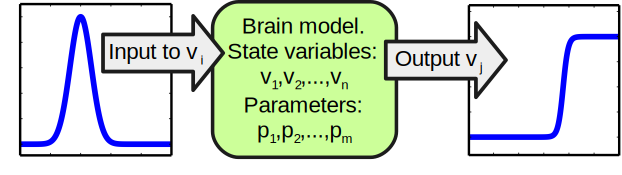
\includegraphics[width=0.9\textwidth]{./figures/intro_graphic.png}
\end{center}
\textbf{\refstepcounter{figure}\label{fig:intro_graphic} Figure \arabic{figure}.}
{ \textbf{fig:intro\_graphic} An isolated brain model. Crafted inputs
are introduced into one of the model's n state variables. The output
of another of the state variables implies behavioural change or
onset.}
\end{figure}

\begin{figure}[htb!]
\begin{center}
\includegraphics[width=0.9\textwidth]{./figures/model_framework.png}
\end{center}
\textbf{\refstepcounter{figure}\label{fig:model_framework} Figure \arabic{figure}.}
{ \textbf{fig:model\_framework} The model framework. The model is specified using a combination of
declarative XML files and hand-coded C++. These original model
specifications are shown within the blue box. b) The green box shows
the processes which are applied to the model specification to produce
the BRAHMS system. Most of the process is defined within the scripts
which make up \stob, but the three hand-written components must be
manually compiled and installed within the BRAHMS Namespace, allowing
the BRAHMS executable to locate them at runtime. c) The red box shows
the resulting BRAHMS system ready to be executed by the BRAHMS
executable. In practice, this call is made by \stob.}
\end{figure}

\begin{figure}[htb!]
\begin{center}
\includegraphics[width=0.9\textwidth]{./figures/mapping.png}
\end{center}
\textbf{\refstepcounter{figure}\label{fig:mapping} Figure \arabic{figure}.}
{ \textbf{fig:mapping} Representative mapping from eye's frame of
reference in cartesian coordinates to retinotopic coordinates. (a) The
mapping of luminances in the eye's frame of reference. The world input
is pre-defined by a JSON configuration file. Luminance position, size
and shape can be defined in this file, along with the times at which
luminances appear and disappear. The worldDataMaker.cpp code computes
the locations of the luminances in the eye's frame of reference, given
its rotational state. It also computes a 2D gaussian convolution of
the luminances. Here, there are two cross shaped luminances spanning
10$\degree$, one of value 0.8 at the fixation point (0,0) and one of
value 0.5 at a peripheral position (0,-12$\degree$). Note that these
crosses have the same `bar width' of 2$\degree$ as the crosses 
used in the simulations, but their span of 10$\degree$ is greater
than the 6$\degree$ used in the simulations, to make these
images clearer. (b) The locations of
the luminances in the eye's frame of reference are then converted into
retinotopic coordinates, with centrally located luminances being
represented at low values of $r$ and more peripheral luminances having
higher values of $r$. $\phi$ encodes rotational angle: 1 and 50 encode
upward movement; 13 is left; 25 is down; 37 is right. The output of
the World component is fed into FEF\_add\_noise and into the retinal
neuron populations. The colour map makes it possible to distinguish
between the two crosses. (c) The FEF\_add\_noise populations adds a level
of noise to the signal representing processing of the signal in visual
cortex. (d) A Gaussian projection from FEF\_add\_noise to FEF further
blurs the activity in FEF. FEF is the input to the basal ganglia and
one input to superior colliculus.}
\end{figure}

\begin{figure}[htb!]
\begin{center}
\includegraphics[width=0.9\textwidth]{./figures/Brain_Model.png}
\end{center}
\textbf{\refstepcounter{figure}\label{fig:brain_model} Figure \arabic{figure}.}
{ \textbf{fig:brain\_model} The brain model. This is the SpineCreator
`network layer' view of the model. Each box represents a neural
population with 2500 elements, arranged in a 50$\times$50 grid. The
SpineML component name is printed on the bottom right corner of each
population box and the population name is at the top. The overall
connectivity between populations is represented by the projection
arrows with the colour indicating the connectivity scheme (one-to-one
connections are red, Gaussian kernel connections are dark blue and so
on). Excitatory connections have arrowheads and inhibitory connections
have circles, although for details of the behaviour of the
connections, the weight-update and post-synapse components must be
studied. Briefly, the model comprises a \e{World} population, into
which a retinotopically organised view of the world is
introduced. This information is passed into cortical populations (FEF)
and subcortical populations (SC) via a simple model of the
retina. These feed a cortico-thalamo-basal ganglia loop, which selects
which region of the deep layer of superior colliculus should be
disinhibited, allowing activity to build up therein. The five
populations comprising the basal ganglia are enclosed in a grey
outline. Note that substantia nigra pars compacta is not modelled
here, instead the level of dopamine in the striatum is set via a
parameter in the Str\_D1 and Str\_D2 populations}
\end{figure}

\begin{figure}[htb!]
\begin{center}
\includegraphics[width=0.5\textwidth]{./figures/Brain_Stem_1channel.png}
\end{center}
\textbf{\refstepcounter{figure}\label{fig:sbg} Figure \arabic{figure}.}
{ \textbf{fig:sbg} One pair of channels of the saccadic burst
generator (SBG) for left (cyan) or right (green) movements. Collicular
activity in SC\_avg excites the channels via SBG weight maps. Each box
represents a neural population and shows the population name, the
number of neural elements (here 2500 or 1) and the SpineML component
name; \e{LIN} for Leaky integrator or \e{integrator}. Key: LLBN:
Long lead burst neurons; IBN: Inhibitory burst neurons; OPN: Omnipause
neurons; EBN: Excitatory burst neurons; TN: Tonic neurons; MN:
Motoneurons.}
\end{figure}

\begin{figure}[htb!]
\begin{center}
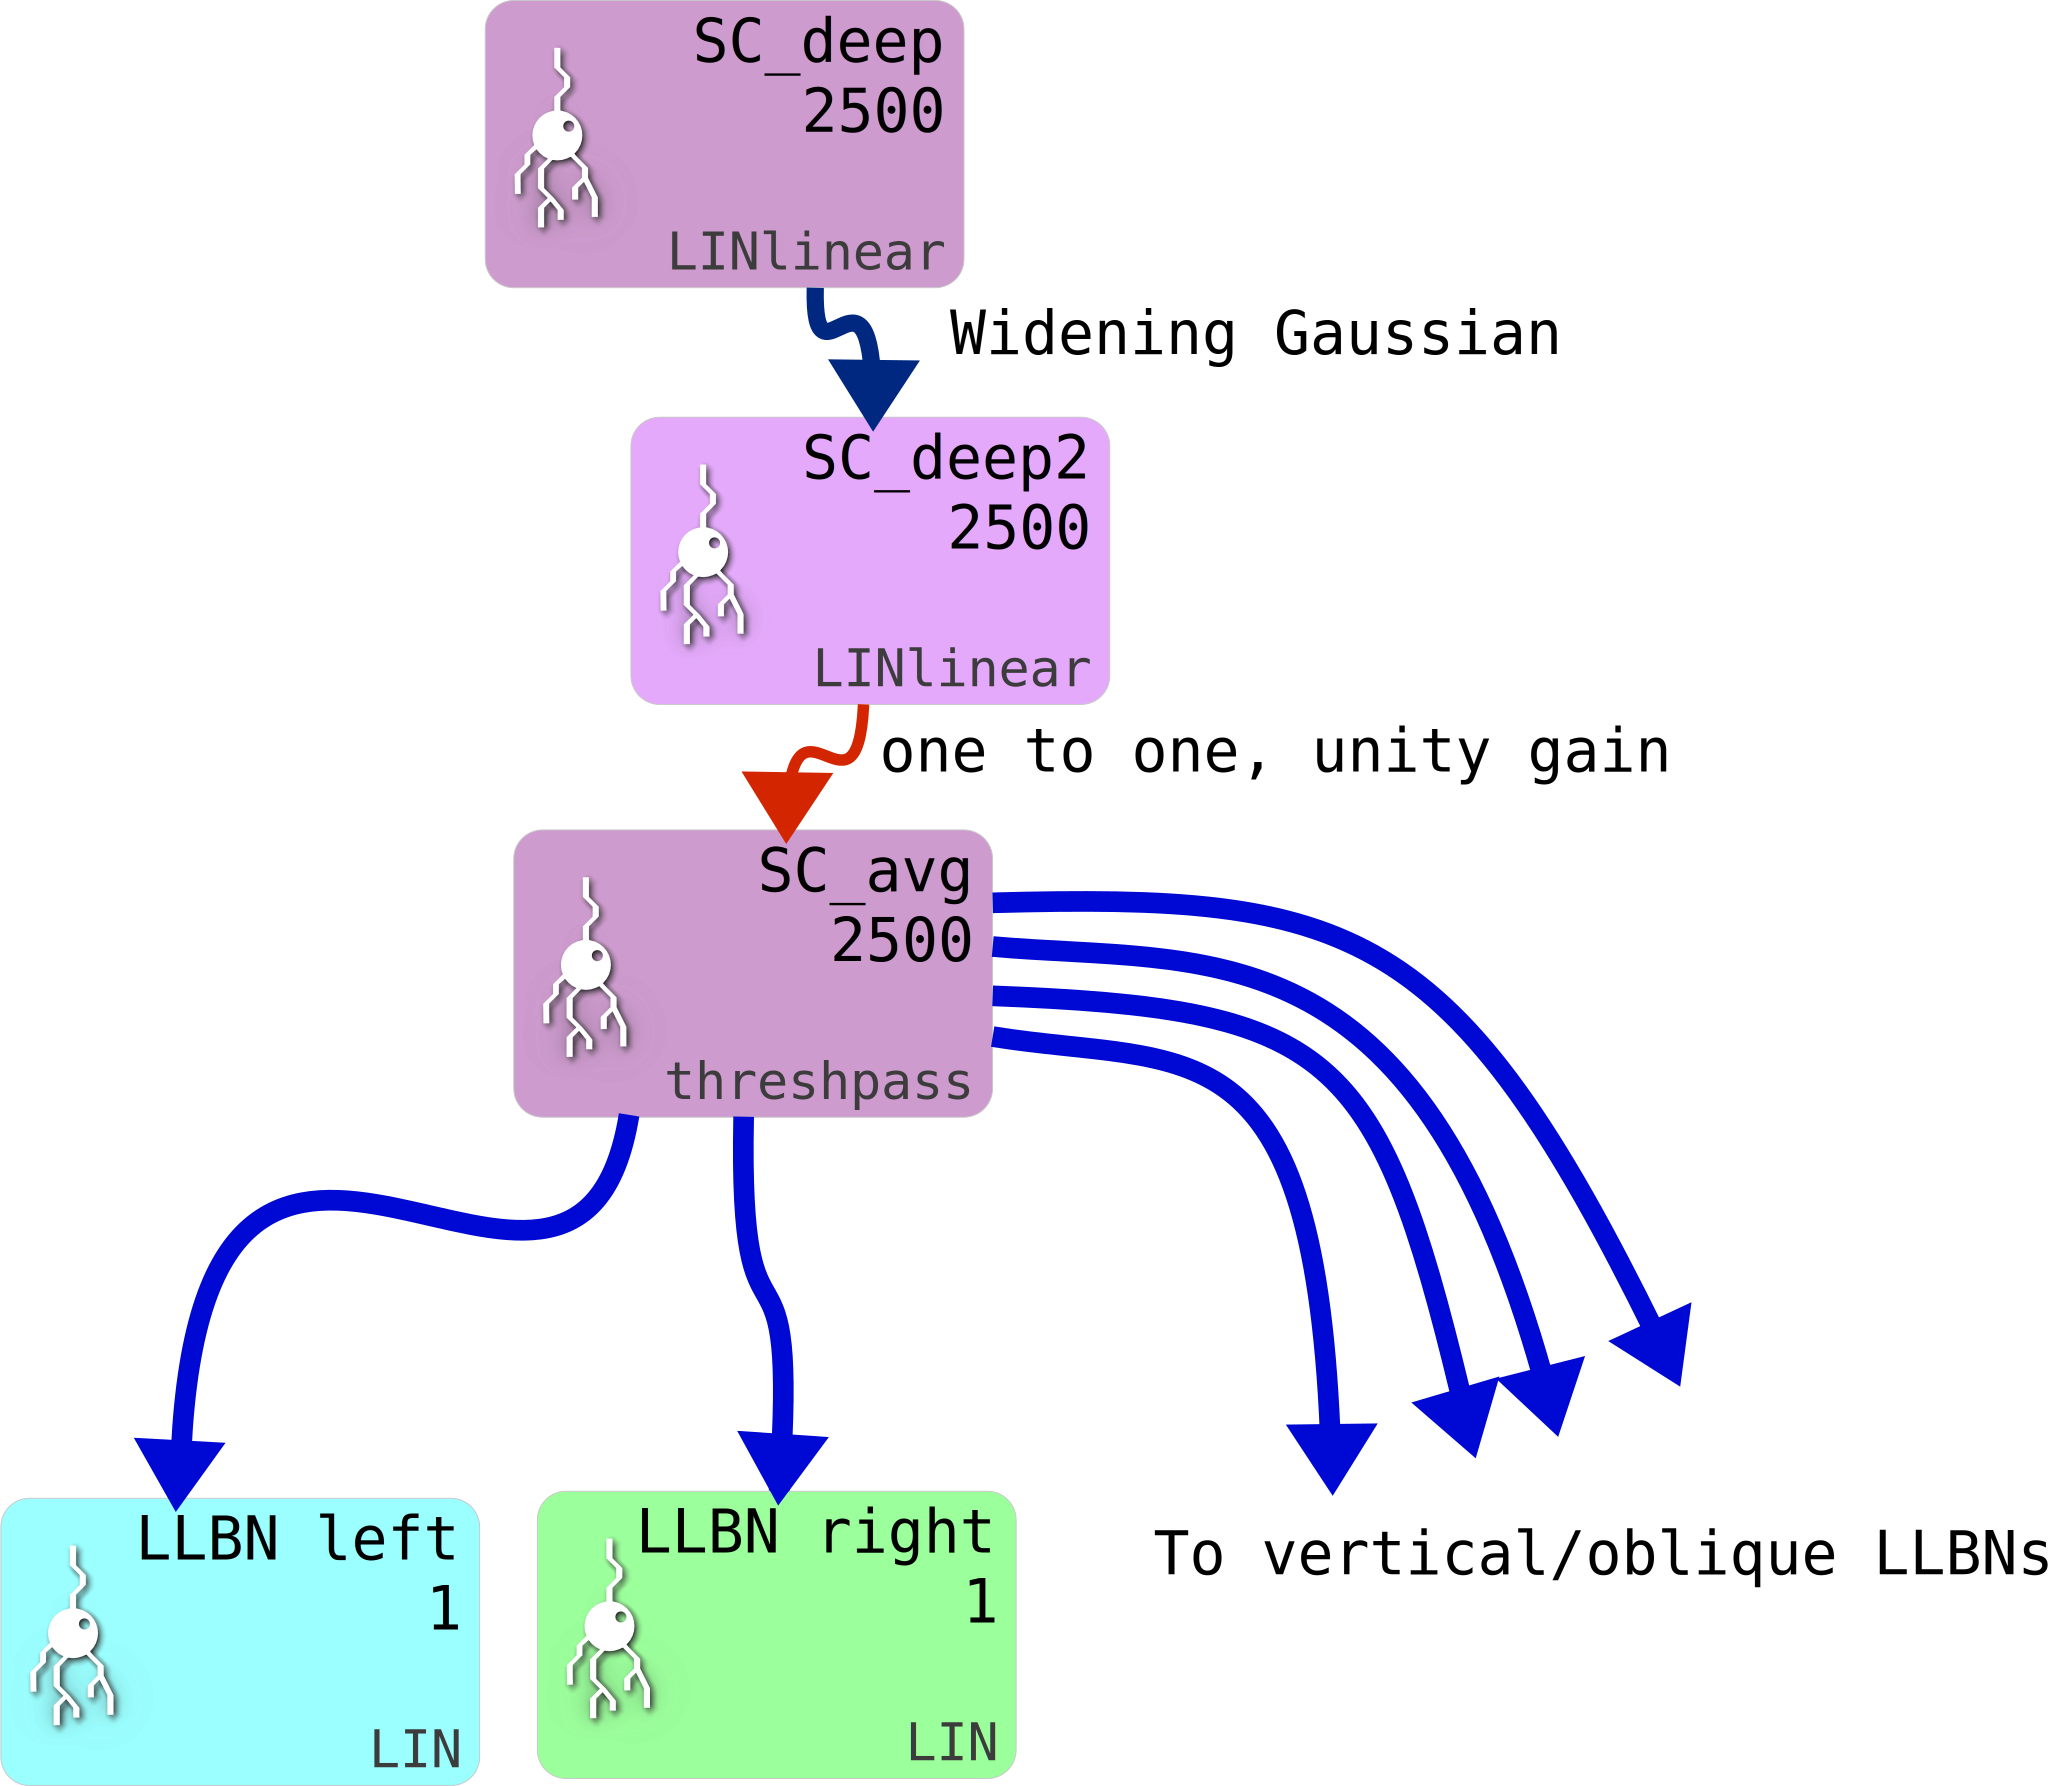
\includegraphics[width=0.5\textwidth]{./figures/SC_to_brainstem.png}
\end{center}
\textbf{\refstepcounter{figure}\label{fig:scdeep} Figure \arabic{figure}.}
{ \textbf{fig:scdeep} Showing additional deep layer of superior colliculus 
(SC\_deep2) and the output layer (SC\_avg, named for the fact that in an earlier
version of the model, it received the output of the centroid of SC\_deep).}
\end{figure}

\begin{figure}[htb!]
\begin{center}
\includegraphics[width=0.8\textwidth]{./figures/sacc_vs_targetpos.png}
\end{center}
\textbf{\refstepcounter{figure}\label{fig:sacc_vs_targ} Figure \arabic{figure}.}
{ \textbf{fig:sacc\_vs\_targ} Accuracy at different target eccentricities for fixation luminance 0.2 and target luminance 0.3.}
\end{figure}

\begin{figure}[htb!]
\begin{center}
\includegraphics[width=\textwidth]{./figures/weightmaps.png}
\end{center}
\textbf{\refstepcounter{figure}\label{fig:weightmaps} Figure \arabic{figure}.}
{ \textbf{fig:weightmaps} Weight maps for the connections between the
output layer of superior colliculus and the six long lead burst
neurons of the saccadic burst generator model. Each map increases
exponentially with increasing $r$, multiplied by cosine($\phi$) about
its `active' axis. \cmnt{Check whether Left \& Right are wrong way round}}
\end{figure}

\begin{figure}[htb!]
\begin{center}
\includegraphics[width=0.8\textwidth]{./figures/outmany.png}
\end{center}
\textbf{\refstepcounter{figure}\label{fig:outmany} Figure \arabic{figure}.}
{ \textbf{fig:outmany} Representative single saccades. a) Trajectories
from 9 saccades to a single target at 9 different locations. In each
case, a fixation cross luminance of magnitude 0.2 was displayed at
(0,0), the start position of the eye, until time 0.4~s. The target
luminance, magnitude 0.3 was illuminated at time 0.4~s. Trajectory
shape is dependent on the target position, and there is a variable
amount of error in the end-points achieved by the model. Colour is
used in this diagram as an aid to distinguishing different saccades
and their targets; for a given saccade, the target location is given
by the cross of the same colour closest to the end of the
trajectory. b) The three rotational components of the `blue' saccade,
to target location (-7,-7). c) The three rotational components of the
`red' saccade, to target location (0,-10).}
\end{figure}

\begin{figure}[htb!]
\begin{center}
\includegraphics[width=0.95\textwidth]{./figures/errorsurface_percent.png}
\end{center}
\textbf{\refstepcounter{figure}\label{fig:errorsurface} Figure \arabic{figure}.}
{ \textbf{fig:errorsurface} The end-point error surface. a) The 
ratio of the magnitudes of the total error vector and the target 
vector, expressed as a percentage. b) The ratio of the magnitude
of the $x$ component of the error vector to the magnitude of the
target vector, expressed as a percentage. c) As (b) but for the
$y$ component. d) As (b), for $z$ component. All colour maps are
shown with the same scale. The target rotations, $\theta_{x}^t$ and
$\theta_{y}^t$ are denoted `Target X' and `Target Y' in the figure.}
\end{figure}

\begin{figure}[htb!]
\begin{center}
\includegraphics[width=0.8\textwidth]{./figures/outrtn.png}
\end{center}
\textbf{\refstepcounter{figure}\label{fig:outrtn} Figure \arabic{figure}.}
{ \textbf{fig:outrtn} There and back - a saccade to a target, followed by return to the original fixation.}
\end{figure}

\begin{figure}[htb!]
\begin{center}
\includegraphics[width=0.8\textwidth]{./figures/lat_vs_everything.png}
\end{center}
\textbf{\refstepcounter{figure}\label{fig:lat_vs_all} Figure \arabic{figure}.}
{ \textbf{fig:lat\_vs\_all} Exploring saccade latencies.}
\end{figure}

\begin{figure}[htb!]
\begin{center}
\includegraphics[width=0.8\textwidth]{./figures/targ_w_distr.png}
\end{center}
\textbf{\refstepcounter{figure}\label{fig:targ_w_distr} Figure \arabic{figure}.}
{ \textbf{fig:targ\_w\_distr} Effect of a distractor on single saccade.}
\end{figure}

\end{document}
